% vim:tw=80:
\documentclass{article}
\usepackage{booktabs}
\usepackage{enumitem}
\usepackage{fancyhdr}
\usepackage[margin=1in]{geometry}
\usepackage{pgfplots}
\usepackage{siunitx}
\usepackage{unicode-math}
\usepackage{hyperref}

\setlist{nosep,listparindent=\parindent}
\pgfplotsset{compat=1.18}

\pagestyle{fancy}
\fancyhf{}
\fancyhead[L]{{{COURSE}}, {{HOMEWORK}}}
\fancyhead[R]{Name: {{AUTHOR}}}
\fancyfoot[C]{\thepage}

\hypersetup{colorlinks=true}

\begin{document}

\begin{center}
  \LARGE {{TITLE}}
\end{center}

\begin{abstract}
  % TODO(algo-hw): state the result quantitatively -- measured exponent per
  % algorithm, speed-up at the largest size both algorithms ran, crossover.
  {{ABSTRACT}}
\end{abstract}

\section{Algorithm Analysis}

% TODO(algo-hw): the exposition of the algorithms, including the recurrence
% and its solution. Fix technical errors; leave the user's voice alone.

\section{Experiment and Results}

We implemented the algorithms in Rust and compared their running times at
different input sizes. The source code was compiled with {{RUSTC}} and the
compiled programs were executed on {{MACHINE}}. The result is shown in
Table~\ref{tab:{{NAME}}-bench} and Figure~\ref{fig:{{NAME}}-bench}.

% TODO(algo-hw): what was measured and how -- release build, size ladder, input
% distribution, the 0.5 s repetition budget, and the check against the naive
% reference.

% Placeholder: `python3 table.py` overwrites this file with the measurements.
\begin{table}[t]
  \centering
  \caption{Placeholder table -- run the benchmark and \texttt{table.py}.}
  \label{tab:{{NAME}}-bench}
  \begin{tabular}{rr}
    \toprule
    $n$ & time (\unit{\milli\second}) \\
    \midrule
    10 & 0.0 \\
    \bottomrule
  \end{tabular}
\end{table}


% Placeholder: `python3 plot.py` overwrites this file with the measurements.
\begin{figure}[t]
  \centering
  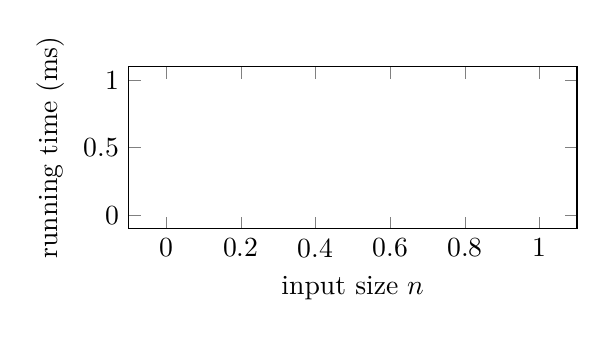
\begin{tikzpicture}
    \begin{axis}[
        width=0.6\textwidth,
        height=0.3\textwidth,
        xlabel={input size $n$},
        ylabel={running time (ms)},
      ]
    \end{axis}
  \end{tikzpicture}
  \caption{Placeholder figure -- run the benchmark and \texttt{plot.py}.}
  \label{fig:{{NAME}}-bench}
\end{figure}


\section{Conclusion}

From the results we conclude the following: \begin{itemize}

  \item TODO(algo-hw): replace with the measured growth per decade or per
    doubling, the fitted exponents, the crossover point, and the explanation
    for the one outlier the data shows.

\end{itemize}

\section*{AI disclosure}

% TODO(algo-hw): list every AI-written artifact -- readme, CLI when the task has
% one, generator, tests, benchmark, plot and table scripts -- plus "reviewed and
% improved this report". The algorithm code is not listed, and the model name
% is left for the user to confirm.
Codex was used to write {{AI_SCOPE}}, to run the experiment, to generate the
result table and figure, and to review and improve this report. The remaining
parts of this work did not involve any use of AI. The workflow behind this
report, including the templates, the benchmark driver and the review
checklist, is packaged as a skill written by the author of this homework:
\url{https://github.com/registerGen/thu/tree/main/26-fall/algo/.agents/skills/algo-hw}.

\end{document}
